\documentclass[11pt,a4paper]{article}
\usepackage[hyperref]{acl2021}
\usepackage{times}
\usepackage{latexsym}
\usepackage{amssymb}
\usepackage{amsmath}
\usepackage{graphicx}
\usepackage{enumitem}
\usepackage{comment}
\usepackage{array}
\usepackage{mathtools}
%\usepackage{booktabs}
\renewcommand{\UrlFont}{\ttfamily\small}

% This is not strictly necessary, and may be commented out,
% but it will improve the layout of the manuscript,
% and will typically save some space.
\usepackage{microtype}

%\aclfinalcopy % Uncomment this line for the final submission
%\def\aclpaperid{***} %  Enter the acl Paper ID here

%\setlength\titlebox{5cm}
% You can expand the titlebox if you need extra space
% to show all the authors. Please do not make the titlebox
% smaller than 5cm (the original size); we will check this
% in the camera-ready version and ask you to change it back.

\newcommand\BibTeX{B\textsc{ib}\TeX}
\DeclareMathOperator*{\argmin}{arg\,min}
\renewcommand\thesection{\Alph{section}}

\title{Appendix}
\date{}
\begin{document}
\section{Convergence of loss during training} 
Figure \ref{fig:train} shows the mean epoch time of SBERT Triplet and SBERT COB on 20NG dataset and CAR dataset (coarse n = 35) respectively.
\begin{figure}[t]
    \centering
    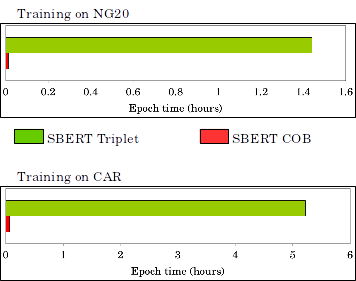
\includegraphics[scale=0.75]{acl-ijcnlp2021-templates/epoch_time.png}
    \caption{Comparison between SBERT COB and SBERT Triplet in terms of epoch time.}
    \label{fig:train}
\end{figure}

\section{Relation between RAND index and Adjacency matrix} Given a set of $n$ data points $\mathcal{P}$, let us compare two clustering results of $\mathcal{P}$, $C_T$ and $C_A$, in terms of RAND index. We know that RAND index is expressed as:
\begin{align*}
    RI &= \frac{a+b}{\binom{n}{2}} \\
    \textrm{where } a &= \textrm{number of pairs that share the same} \\ 
    & \quad \textrm{cluster both in $C_T$ and $C_A$} \\
    \textrm{where } b &= \textrm{number of pairs that are from different} \\
    & \quad \textrm{clusters both in $C_T$ and $C_A$}
\end{align*}
Now we can express any clustering result $C_M$ in form of an adjacency matrix $M$ where $M_{ij}=1$ if the $i,j$-th data points in $\mathcal{P}$ share the same cluster in $C_M$ and $M_{ij}=0$ otherwise. We represent the clustering results $C_T$ and $C_A$ with such adjacency matrices $T$ and $A$ respectively. Also, the difference matrix of $A,T$ denoted as $|A-T|$ indicates the ordered pairs that do not agree between $A,T$. In other words, $|A_{ij}-T_{ij}|=1$ denotes that the $i,j$-th data points do not agree between $A$ and $T$. Now, we can express RAND index in terms of $A$ and $T$ as follows:

\begin{align*}
    RI &= \frac{a+b}{\binom{n}{2}} \\
    &= \frac{\text{No. of agreements between } C_T,C_A}{\binom{n}{2}} \\
    &= \frac{\parbox{0.9\linewidth}{No. of unordered pairs in $\mathcal{P}$ that agrees between $C_T,C_A$}}{\binom{n}{2}} \\
    &= \frac{\parbox{0.9\linewidth}{No. of ordered pairs in $\mathcal{P}$ that agrees between $C_T,C_A$}}{2\binom{n}{2}} \\
    &= \frac{\text{Total ordered pairs in $\mathcal{P}$}-\sum_{ij} |A_{ij}-T_{ij}|}{2\binom{n}{2}} \\
    &= \frac{2\binom{n}{2}-\sum_{ij} |A_{ij}-T_{ij}|}{2\binom{n}{2}} \\
    &= 1-\frac{\sum_{ij} |A_{ij}-T_{ij}|}{2\binom{n}{2}}
\end{align*}

\end{document}
